
% RUN:
% pdflatex -output-directory=/Users/salvatorpes/Desktop/Aprendizagem/Homework3/trash /Users/salvatorpes/Desktop/Aprendizagem/Homework3/G022.tex

% ir a settings.json e adicionar:
% // According to the wiki, the string latex-workshop.latex.autoBuild.run has three possible values: never, onSave and onFileChange(default).
% "latex-workshop.latex.autoBuild.run": "never",

\documentclass{article}


\author{Pedro Curvo (ist1102716) $|$ Salvador Torpes (ist1102474)}

\usepackage[utf8]{inputenc}
\usepackage[english]{babel}
% \usepackage[letterpaper,top=10mm,bottom=15mm,left=15mm,right=15mm,marginparwidth=1.75cm]{geometry}
% \usepackage[letterpaper,top=10mm,bottom=15mm,left=15mm,right=15mm,marginparwidth=1.75cm]{geometry}
\usepackage[letterpaper,margin=1in,marginparwidth=1.75cm]{geometry}
\usepackage{multicol}
\usepackage{biblatex}
\usepackage{cancel}
\usepackage{colortbl}
\addbibresource{Bibliografia.bib}
\usepackage{graphicx}
% \graphicspath{{../Homework1/images/}}
\usepackage{subcaption}
\usepackage{tabularx}
\usepackage{ulem}
\usepackage{booktabs}
\usepackage{array}
\usepackage{makecell}
\usepackage{multirow}
\usepackage{amsmath}
\usepackage{makecell}
\usepackage{url}
\usepackage{csquotes}
\usepackage{caption}
\usepackage{enumitem}
\usepackage{textcomp}
\usepackage{pdflscape}
\usepackage{makeidx}
\usepackage{amsmath}
% \usepackage{tocbibind}
\providecommand{\tightlist}{\relax}
\usepackage{tocloft}
\renewcommand{\cftsecindent}{0em}
\renewcommand{\cftsubsecindent}{1em}
\renewcommand{\cftsecfont}{\bfseries}
\renewcommand{\cftsubsecfont}{\itshape}
\setlength{\cftsubsecnumwidth}{0em}

\usepackage[version=4]{mhchem}
\usepackage{hyperref} % Remove "pdftex" option here
\usepackage{float}
\usepackage{fancyhdr}
\usepackage{ragged2e}
\usepackage{xkeyval}
%\usepackage{minted}
%\usemintedstyle{manni}
\usepackage{listings}
\usepackage{amssymb}




\usepackage{tikz}
\usetikzlibrary{positioning}
\usetikzlibrary{positioning, arrows.meta}
\usepackage{adjustbox}
\usepackage{sidecap}



% \usepackage[table,xcdraw]{xcolor}
\usepackage[LY1]{fontenc}
\usepackage{tikz-3dplot}
% \usepackage{pgfplots}
\usetikzlibrary{calc, 3d, arrows}
\usepackage{forest}




\usetikzlibrary{shapes.geometric, arrows}


\lstset{
    language=Python,
    basicstyle=\ttfamily,
    keywordstyle=\color{blue},
    commentstyle=\color{gray},
    stringstyle=\color{orange},
    numbers=left,
    numberstyle=\tiny,
    numbersep=5pt,
    showspaces=false,
    showstringspaces=false,
    breaklines=true,
    frame=tb,
    framexleftmargin=2em,
    xleftmargin=2em,
}


%\usepackage{fontspec}

%\setmonofont{Fira Code}

\fancyhf{}
\cfoot{\thepage}
\fancyhf{} % Clear all header and footer fields
\renewcommand{\headrulewidth}{0pt} % Remove the header rule line
\cfoot{\thepage} % Set the page number in the center of the footer

\pagestyle{fancy} % Apply the fancy page style

\setlength\columnsep{20pt}

\renewcommand{\familydefault}{\sfdefault}

\newenvironment{Figure}
  {\par\medskip\noindent\minipage{\linewidth}}
  {\endminipage\par\medskip}

\makeatletter
\newenvironment{figurehere}
{\def\@captype{figure}}
{}
\makeatother

\hypersetup{
  colorlinks,
  linkcolor=blue,
  anchorcolor=black,
  citecolor=cyan,
  filecolor=cyan,
  menucolor=cyan,
  urlcolor=cyan,
  bookmarksopen=true,
  bookmarksnumbered=true
}

\makeindex


\title{\vspace{-6mm}
\includegraphics[width=15mm,scale=2]{images/IST_Logo.png}\\ \vspace{5mm}
Machine Learning - Homework 3 \vspace{-5mm}}
\date{1st Term - 23/24}

\usepackage{sansmathfonts}
\usepackage[T1]{fontenc}
\usepackage[OT1]{fontenc}

\usepackage{listings}
\usepackage{xcolor}

\definecolor{codegreen}{rgb}{0,0.6,0}
\definecolor{codegray}{rgb}{0.5,0.5,0.5}
\definecolor{codepurple}{rgb}{0.58,0,0.82}
\definecolor{backcolour}{rgb}{0.95,0.95,0.92}

\lstdefinestyle{mystyle}{
  backgroundcolor=\color{backcolour},   
  commentstyle=\color{codegray},
  keywordstyle=\color{magenta},
  numberstyle=\tiny\color{codegray},
  stringstyle=\color{codegreen},
  keywordstyle=[2]{\color{orange}},
  keywords=[2]{plt.},
  basicstyle=\ttfamily\footnotesize,
  breakatwhitespace=false,         
  breaklines=true,                 
  captionpos=b,                    
  keepspaces=true,                 
  numbers=left,                    
  numbersep=5pt,                  
  showspaces=false,                
  showstringspaces=false,
  showtabs=false,                  
  tabsize=2,
  frame=single,
  framesep=2pt,
  framerule=0pt,
  xleftmargin=2pt,
  xrightmargin=2pt,
  aboveskip=1em,
  belowskip=1em,
  abovecaptionskip=0.5em,
  belowcaptionskip=0.5em,
  caption=\lstname,
  captionpos=b,
  language=Python,
  morekeywords={as},
  deletekeywords={None},
  emph={self},
  emphstyle=\color{blue},
  escapeinside={(*@}{@*)},
  literate={+}{{\textcolor{blue}{+}}}1
       {*}{{\textcolor{blue}{*}}}1
       {-}{{\textcolor{blue}{-}}}1
       {/}{{\textcolor{blue}{/}}}1
       {=}{{\textcolor{blue}{=}}}1
       {>}{{\textcolor{blue}{>}}}1
       {<}{{\textcolor{blue}{<}}}1
       {==}{{\textcolor{blue}{==}}}2
       {!=}{{\textcolor{blue}{!=}}}2
       {<=}{{\textcolor{blue}{<=}}}2
       {>=}{{\textcolor{blue}{>=}}}2,
  }
    
    \lstset{style=mystyle}
    \usepackage{fancyhdr}
    
    % Define header and footer styles
    \fancypagestyle{plain}{%
      \fancyhf{}% Clear header/footer
      \fancyhead[L]{Homework 3}% Header left
      \fancyhead[C]{2023/2024}% Header left
      \fancyhead[R]{Machine Learning}% Header right
      \fancyfoot[C]{\thepage}% Footer center
      \renewcommand{\headrulewidth}{0.4pt}% Header rule
      \renewcommand{\footrulewidth}{0pt}% Footer rule
    }
    
    % Apply the style to all pages except the first one
    \pagestyle{plain}
    \thispagestyle{empty} % Remove header/footer from first page


    \usepackage{amsmath} % for aligned
    %\usepackage{amssymb} % for \mathbb
    \usepackage{tikz}
    %\usepackage{etoolbox} % for \ifthen
    \usepackage{listofitems} % for \readlist to create arrays
    \usetikzlibrary{arrows.meta} % for arrow size
    \usepackage[outline]{contour} % glow around text
    \contourlength{1.4pt}
    
    \tikzset{>=latex} % for LaTeX arrow head
    \usepackage{xcolor}
    \colorlet{myred}{red!80!black}
    \colorlet{myblue}{blue!80!black}
    \colorlet{mygreen}{green!60!black}
    \colorlet{myyellow}{yellow!80!black}
    \colorlet{myorange}{orange!70!red!60!black}
    \colorlet{mydarkred}{red!30!black}
    \colorlet{mydarkblue}{blue!1!black}
    \colorlet{mydarkgreen}{green!30!black}
    \tikzstyle{node}=[thick,circle,draw=myblue,minimum size=22,inner sep=0.5,outer sep=0.6]
    \tikzstyle{node in}=[node,green!20!black,draw=mygreen!30!black,fill=myyellow!25]
    \tikzstyle{node hidden}=[node,blue!20!black,draw=myblue!30!black,fill=myorange!55]
    \tikzstyle{node convol}=[node,orange!20!black,draw=myorange!30!black,fill=myorange!20]
    \tikzstyle{node out}=[node,red!20!black,draw=myred!30!black,fill=myred!20]
    \tikzstyle{connect}=[thick,mydarkred] %,line cap=round
    \tikzstyle{connect arrow}=[-{Latex[length=4,width=3.5]},thick,mydarkblue,shorten <=0.5,shorten >=1]
    \tikzset{ % node styles, numbered for easy mapping with \nstyle
      node 1/.style={node in},
      node 2/.style={node hidden},
      node 3/.style={node out},
    }
    \def\nstyle{int(\lay<\Nnodlen?min(2,\lay):3)} % map layer number onto 1, 2, or 3


\begin{document}
    
\renewcommand{\arraystretch}{1.7}
\setlength{\columnseprule}{0.4pt}
\tdplotsetmaincoords{70}{110} % Set the viewing angle
\newcolumntype{M}[1]{>{\centering\arraybackslash\vspace{#1}}m{0.5\linewidth}<{\vspace{#1}}}
\newcolumntype{C}[2]{>{\centering\arraybackslash\vspace{#1}\rule{0pt}{#1}\hspace{0pt}}m{#2}}
\ifx\undefined\w
\newcolumntype{w}[1]{>{\centering\arraybackslash}m{#1}}
\fi
\renewcommand*\familydefault{\sfdefault} %% Only if the base font of the document is to be sans serif

% NEURAL NETWORK with coefficients, uniform arrows
\newcommand\setAngles[3]{
  \pgfmathanglebetweenpoints{\pgfpointanchor{#2}{center}}{\pgfpointanchor{#1}{center}}
  \pgfmathsetmacro\angmin{\pgfmathresult}
  \pgfmathanglebetweenpoints{\pgfpointanchor{#2}{center}}{\pgfpointanchor{#3}{center}}
  \pgfmathsetmacro\angmax{\pgfmathresult}
  \pgfmathsetmacro\dang{\angmax-\angmin}
  \pgfmathsetmacro\dang{\dang<0?\dang+360:\dang}
}

\maketitle
\vspace{-5mm}
\hrulefill




\section*{Pen and Paper Exercises}

\section*{1\textsuperscript{st} Question}

\subsection*{Dataset}

In this exercise we aim to learn a regression model for the following dataset:

\begin{table}[H]
    \centering
    \begin{tabular}{|c|c|c|c|c|}
        \hline
        Observation     & $x_0$ & $x_1$ & $x_2$ & output - $z$ \\ \hline
        $\vec{x}_1$               & 1     & 0.7   & -0.3  & 0.8           \\ \hline
        $\vec{x}_2$               & 1     & 0.4   & 0.5   & 0.6           \\ \hline
        $\vec{x}_3$               & 1     & -0.2  & 0.8   & 0.3           \\ \hline
        $\vec{x}_4$               & 1     & -0.4  & 0.3   & 0.3           \\ \hline
    \end{tabular}
    \caption{Dataset}
    \label{tab:my_label}
\end{table}

\[ X = \begin{bmatrix} 1 & 0.7 & -0.3 \\ 1 & 0.4 & 0.5 \\ 1 & -0.2 & 0.8 \\ 1 & -0.4 & 0.3 \end{bmatrix} \qquad Z = \begin{bmatrix} 0.8 \\ 0.6 \\ 0.3 \\ 0.3 \end{bmatrix} \]
\[ \vec{x}_1 = \begin{bmatrix} 0.7 \\ -0.3 \end{bmatrix} \qquad \vec{x}_2 = \begin{bmatrix} 0.4 \\ 0.5 \end{bmatrix} \qquad \vec{x}_3 = \begin{bmatrix} -0.2 \\ 0.8 \end{bmatrix} \qquad \vec{x}_4 = \begin{bmatrix} -0.4 \\ 0.3 \end{bmatrix} \]

\subsection*{a)}

\subsubsection*{Transforming the data}

We are transforming our original data into a new space, according to the radial basis function:

\[ \phi_j(\vec{x}) = \exp \left( - \frac{||\vec{x} - c_j||^2}{2} \right) \]

\[ c_1 = \begin{bmatrix} 0 \\ 0 \end{bmatrix} \qquad c_2 = \begin{bmatrix} 1 \\ -1 \end{bmatrix} \qquad c_3 = \begin{bmatrix} -1 \\ 1 \end{bmatrix} \]

After applying the transformation, we will have 3 new inputs for each observation. Therefore, the new dataset will look like:

\[ \Phi(X) =  X_{trans} = \begin{bmatrix} 1 & \phi_1(\vec{x}_1) & \phi_2(\vec{x}_1) & \phi_3(\vec{x}_1) \\ 1 & \phi_1(\vec{x}_2) & \phi_2(\vec{x}_2) & \phi_3(\vec{x}_2) \\ 1 & \phi_1(\vec{x}_3) & \phi_2(\vec{x}_3) & \phi_3(\vec{x}_3) \\ 1 & \phi_1(\vec{x}_4) & \phi_2(\vec{x}_4) & \phi_3(\vec{x}_4) \end{bmatrix} \]

\paragraph{Observation 1}

If we apply our transformation to the first observation $\vec{x}_1$, we get:

\[ \phi_1(\vec{x}_1) = \exp \left( - \frac{||\vec{x}_1 - c_1||^2}{2} \right) = \exp \left( - \frac{0.58}{2} \right) = 0.74826 \]

\[ \phi_2(\vec{x}_1) = \exp \left( - \frac{||\vec{x}_1 - c_2||^2}{2} \right) = \exp \left( - \frac{0.58}{2} \right) = 0.74826 \]

\[ \phi_3(\vec{x}_1) = \exp \left( - \frac{||\vec{x}_1 - c_3||^2}{2} \right) = \exp \left( - \frac{4.58}{2} \right) = 0.10127 \]

\paragraph{Observation 2}

If we apply our transformation to the second observation $\vec{x}_2$, we get:

\[ \phi_1(\vec{x}_2) = \exp \left( - \frac{||\vec{x}_2 - c_1||^2}{2} \right) = \exp \left( - \frac{0.41}{2} \right) = 0.81465 \]

\[ \phi_2(\vec{x}_2) = \exp \left( - \frac{||\vec{x}_2 - c_2||^2}{2} \right) = \exp \left( - \frac{2.61}{2} \right) = 0.27117 \]

\[ \phi_3(\vec{x}_2) = \exp \left( - \frac{||\vec{x}_2 - c_3||^2}{2} \right) = \exp \left( - \frac{2.21}{2} \right) = 0.33121 \]

\paragraph{Observation 3}

If we apply our transformation to the third observation $\vec{x}_3$, we get:

\[ \phi_1(\vec{x}_3) = \exp \left( - \frac{||\vec{x}_3 - c_1||^2}{2} \right) = \exp \left( - \frac{0.68}{2} \right) = 0.71177 \]

\[ \phi_2(\vec{x}_3) = \exp \left( - \frac{||\vec{x}_3 - c_2||^2}{2} \right) = \exp \left( - \frac{4.68}{2} \right) = 0.09633 \]

\[ \phi_3(\vec{x}_3) = \exp \left( - \frac{||\vec{x}_3 - c_3||^2}{2} \right) = \exp \left( - \frac{0.68}{2} \right) = 0.71177 \]

\paragraph{Observation 4}

If we apply our transformation to the fourth observation $\vec{x}_4$, we get:

\[ \phi_1(\vec{x}_4) = \exp \left( - \frac{||\vec{x}_4 - c_1||^2}{2} \right) = \exp \left( - \frac{0.25}{2} \right) = 0.88250 \]

\[ \phi_2(\vec{x}_4) = \exp \left( - \frac{||\vec{x}_4 - c_2||^2}{2} \right) = \exp \left( - \frac{3.65}{2} \right) = 0.16122 \]

\[ \phi_3(\vec{x}_4) = \exp \left( - \frac{||\vec{x}_4 - c_3||^2}{2} \right) = \exp \left( - \frac{0.85}{2} \right) = 0.65377 \]

\subsubsection*{Transformed Dataset}

After applying the transformation, we get the following dataset:

\[ \Phi(X) = X_{trans} = \begin{bmatrix}
    1 & 0.74826 & 0.74826 & 0.10127 \\
    1 & 0.81465 & 0.27117 & 0.33121 \\
    1 & 0.71177 & 0.09633 & 0.71177 \\
    1 & 0.88250 & 0.16122 & 0.65377
\end{bmatrix} \]

\begin{table}[H]
    \centering
    \begin{tabular}{|c|c|c|c|c|c|}
        \hline
        Observation     & $\phi_0$ & $\phi_1$ & $\phi_2$ & $\phi_3$ & output - $z$ \\ \hline
        $\vec{x}_1$               & 1     & 0.74826   & 0.74826  & 0.10127 & 0.8           \\ \hline
        $\vec{x}_2$               & 1     & 0.81465   & 0.27117   & 0.33121  & 0.6           \\ \hline
        $\vec{x}_3$               & 1     & 0.71177  & 0.09633   & 0.71177   & 0.3           \\ \hline
        $\vec{x}_4$               & 1     & 0.88250  & 0.16122   & 0.65377   & 0.3           \\ \hline
    \end{tabular}
    \caption{Transformed Dataset}
    \label{tab:my_label}
\end{table}

\subsubsection*{Ridge Regression}

A regression model is characterized by a column matrix of weights $W$ - if we multiply $W$ by a new observation, we get the estimated output for that observation.

\[ \hat{z} = w_0 + \sum_{j=1}^{M} w_j x_j = X \cdot W \]

$X$ is the matrix of observations, and $W$ is the matrix of weights:

\[ X = \begin{bmatrix} 1 & \vec{x}_1^T \\ 1 & \vec{x}_2^T \\ 1 & \vec{x}_3^T \\ 1 & \vec{x}_4^T \end{bmatrix} \qquad W = \begin{bmatrix} w_0 \\ w_1 \\ w_2 \\ w_3 \end{bmatrix} \]

When considering the case where we \textbf{transform} our data according to a function $\phi$, the regression formula is:

\[ \hat{z} = w_0 + \sum_{j=1}^{M} w_j \phi_j(x) = \Phi(X) \cdot W \]

The Ridge Regression ($l_2$ regularization) is a method that penalizes the weights of the model, in order to avoid overfitting. The formula for $W$ matrix in the Ridge Regression is:

\[ W = ( \Phi^T \Phi + \lambda I )^{-1} \Phi^T Z \]

Where $\lambda$ is the regularization parameter ($\lambda = 0.1$), $I$ is the identity matrix and $\Phi$ is the matrix of transformed observations.

\subsubsection*{Computing the weights}

Using the formula for $W$, we get:

\[ 
    \Phi = \begin{bmatrix}
    1 & 0.74826 & 0.74826 & 0.10127 \\
    1 & 0.81465 & 0.27117 & 0.33121 \\
    1 & 0.71177 & 0.09633 & 0.71177 \\
    1 & 0.88250 & 0.16122 & 0.65377
\end{bmatrix} 
\qquad 
Z = \begin{bmatrix} 0.8 \\ 0.6 \\ 0.3 \\ 0.3 \end{bmatrix} \
\qquad 
\Phi^T = \begin{bmatrix}
    1 & 1 & 1 & 1 \\
    0.74826 & 0.81465 & 0.71177 & 0.88250 \\
    0.74826 & 0.27117 & 0.09633 & 0.16122 \\
    0.10127 & 0.33121 & 0.71177 & 0.65377
\end{bmatrix} \]

\[ (\Phi^T \Phi - \lambda I)^{-1} = \begin{bmatrix}
    4.54826  & -3.77682 & -1.86117 & -1.86155 \\
    -3.77682 & 5.98285  & -0.88543 & -1.26432 \\
    -1.86117 & -0.88543 &  4.33276 &  2.72156 \\
    -1.86155 & -1.26432 &  2.72156 &  4.53204 \\
\end{bmatrix} \]

\[ W = (\Phi^T \Phi + \lambda I)^{-1} \Phi^T Z = \begin{bmatrix} w_0 \\ w_1 \\ w_2 \\ w_3 \end{bmatrix} = \begin{bmatrix} 0.33914 \\ 0.19945 \\ 0.40096 \\ -0.29600 \end{bmatrix} \]

\subsubsection*{Final form of the prediction function}

In order to compute $\hat{z}$, we need to multiply the weights by the transformed observation:

\[ \hat{z} = \sum_{j=0}^{3} w_j \phi_j(x) = \Phi(X) \cdot W  \Leftrightarrow \]
\[ \Leftrightarrow \hat{z} = w_0 + w_1 \cdot \phi_1 + w_2 \cdot \phi_2 + w_3 \cdot \phi_3 = 0.33914 + 0.19945 \cdot \phi_1 + 0.40096 \cdot \phi_2 - 0.29600 \cdot \phi_3 \]

\paragraph{}
Using our dataset, the predicted values are:

\[ \hat{z} = \begin{bmatrix}
    0.75844 \\
    0.51232 \\
    0.30905 \\
    0.38629
\end{bmatrix} \]

\subsection*{b)}

The RMSE (Root Mean Squared Error) is a metric that measures the difference between the predicted values and the actual values. It is defined as:

\[ RMSE = \sqrt{\frac{1}{N} \sum_{i=1}^{N} (z_i - \hat{z}_i)^2} \]

Where $z_i$ is the actual value and $\hat{z}_i$ is the predicted value.
In our case, we have the following data:

\begin{table}[H]
    \centering
    \begin{tabular}{|c|c|}
        \hline
        $z_i$ & $\hat{z}_i$ \\ \hline
        0.8   & 0.75844     \\ \hline
        0.6   & 0.51232     \\ \hline
        0.3   & 0.30905     \\ \hline
        0.3   & 0.38629     \\ \hline
    \end{tabular}
    \caption{Actual and Predicted Values}
    \label{tab:my_label}
\end{table}

The RMSE is:

\[ RMSE = \sqrt{\frac{1}{4} \sum_{i=1}^{4} (z_i - \hat{z}_i)^2} = \sqrt{\frac{1}{4} \cdot 0.01694} = 0.06508 \]


\newpage

\section*{2\textsuperscript{nd} Question}

\subsection*{Structure of the Network}

We are considering a MLP (Multi-Layer Perceptron) with 2 hidden layers. The input and output layers each have 3 neurons. 
Our structure is the following:

\begin{center}
% NEURAL NETWORK with coefficients, no arrows
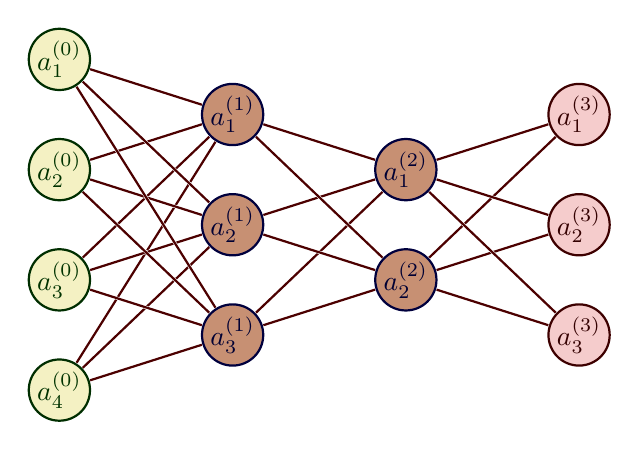
\begin{tikzpicture}[x=2.2cm,y=1.4cm]
\message{^^JNeural network without arrows}
\readlist\Nnod{4,3,2,3} % array of number of nodes per layer

\message{^^J  Layer}
\foreachitem \N \in \Nnod{ % loop over layers
    \def\lay{\Ncnt} % alias of index of current layer
    \pgfmathsetmacro\prev{int(\Ncnt-1)} % number of previous layer
    \message{\lay,}
    \foreach \i [evaluate={\y=\N/2-\i; \x=\lay; \n=\nstyle;}] in {1,...,\N}{ % loop over nodes
    
    % NODES
    \node[node \n] (N\lay-\i) at (\x,\y) {$a_\i^{(\prev)}$};
    
    % CONNECTIONS
    \ifnum\lay>1 % connect to previous layer
        \foreach \j in {1,...,\Nnod[\prev]}{ % loop over nodes in previous layer
        \draw[connect,white,line width=1.2] (N\prev-\j) -- (N\lay-\i);
        \draw[connect] (N\prev-\j) -- (N\lay-\i);
        %\draw[connect] (N\prev-\j.0) -- (N\lay-\i.180); % connect to left
        }
    \fi % else: nothing to connect first layer
    
    }
}

% LABELS
% \node[above=5,align=center,mygreen!60!black] at (N1-1.90) {input\\[-0.2em]layer};
% \node[above=2,align=center,myblue!60!black] at (N3-1.90) {hidden layer};
% \node[above=8,align=center,myred!60!black] at (N\Nnodlen-1.90) {output\\[-0.2em]layer};

\end{tikzpicture}
\end{center}

\subsection*{Activation Function}

The activation function is the hyperbolic tangent function and it is the same for all layers:

\[ \Phi(x) = f(x) = \tanh(0.5x-2) \]

\[ \Phi'(x) = f'(x) = \frac{0.5}{\cosh^2(0.5x-2)} =0.5 \cdot \left( 1 - \tanh^2(0.5x-2) \right) = 0.5 \cdot \left( 1 - \Phi^2(x) \right) \]

\subsection*{Loss Function}

The loss function is the mean square error:

\[ E(W) = \frac{1}{2} \sum_{i=1}^{N} ||z_i - \hat{z}_i||^2 \]

\subsection*{Initial Weights}

We are told the initial weights are:

\[ w^{[1]} = \begin{bmatrix} 1 & 1 & 1 & 1 \\ 1 & 1 & 2 & 1 \\ 1 & 1 & 1 & 1 \end{bmatrix} \qquad w^{[2]} = \begin{bmatrix} 1 & 4 & 1 \\ 1 & 1 & 1 \end{bmatrix} \qquad w^{[3]} = \begin{bmatrix} 1 & 1  \\ 3 & 1 \\ 1 & 1 \end{bmatrix} \]
\[ b^{[1]} = \begin{bmatrix} 1 \\ 1 \\ 1 \end{bmatrix} \qquad b^{[2]} = \begin{bmatrix} 1 \\ 1 \end{bmatrix} \qquad b^{[3]} = \begin{bmatrix} 1 \\ 1 \\ 1 \end{bmatrix} \]

According to these weights, we can compute the initial values for $X^{[1]}$, $X^{[2]}$ and $X^{[3]}$. 
We are considering two training observations and therefore have two different $X^{[0]}$ vectors:

\[ X^{[0]}_1 = \begin{bmatrix} 1 \\ 1 \\ 1 \\ 1  \end{bmatrix} \qquad X^{[0]}_2 = \begin{bmatrix} 1 \\ 0 \\ 0 \\ -1  \end{bmatrix} \]

With $X^{[0]}$ we can compute $X^{[1]}$, $X^{[2]}$ and $X^{[3]}$ - Propagation of both inputs through the network:

\[ X^{[1]}_1 = \Phi(W^{[1]} \cdot X^{[0]}_1 + b^{[1]}) = \tanh \left( \left(\begin{bmatrix} 1 & 1 & 1 & 1 \\ 1 & 1 & 2 & 1 \\ 1 & 1 & 1 & 1 \end{bmatrix} \cdot \begin{bmatrix} 1 \\ 1 \\ 1 \\ 1 \end{bmatrix} + \begin{bmatrix} 1 \\ 1 \\ 1 \end{bmatrix} \right) \cdot 0.5 - 2I \right) = \tanh \left( \begin{bmatrix} 0.5 \\ 1 \\ 0.5 \end{bmatrix} \right)  = \begin{bmatrix} 0.46212 \\ 0.76159 \\ 0.46212 \end{bmatrix} \]

\[ Z^{[1]}_1 = W^{[1]} \cdot X^{[0]}_1 + b^{[1]} = \begin{bmatrix} 5 \\ 6 \\ 5 \end{bmatrix} \]

\[ X^{[2]}_1 = \Phi(W^{[2]} \cdot X^{[1]}_1 + b^{[2]}) = \tanh \left( \left(\begin{bmatrix} 1 & 4 & 1 \\ 1 & 1 & 1 \end{bmatrix} \cdot \begin{bmatrix} 0.46212 \\ 0.76159 \\ 0.46212 \end{bmatrix} + \begin{bmatrix} 1 \\ 1 \end{bmatrix} \right) \cdot 0.5 - 2I \right) = \tanh \left( \begin{bmatrix} 0.45048 \\ -0.57642 \end{bmatrix} \right)  = \begin{bmatrix} 0.45048 \\ -0.57642 \end{bmatrix} \]

\[ Z^{[2]}_1 = W^{[2]} \cdot X^{[1]}_1 + b^{[2]} = \begin{bmatrix} 4.97061 \\ 2.68583 \end{bmatrix} \]

\[ X^{[3]}_1 = \Phi(W^{[3]} \cdot X^{[2]}_1 + b^{[3]}) = \tanh \left( \left(\begin{bmatrix} 1 & 1  \\ 3 & 1 \\ 1 & 1 \end{bmatrix} \cdot \begin{bmatrix} -0.9159 \\ -0.80494 \end{bmatrix} + \begin{bmatrix} 1 \\ 1 \\ 1 \end{bmatrix} \right) \cdot 0.5 - 2I \right) = \tanh \left( \begin{bmatrix} -1.56297 \\ -1.11249 \\ -1.56297 \end{bmatrix} \right)  = \begin{bmatrix} -0.9159 \\ -0.80494 \\ -0.9159 \end{bmatrix} \]

\[ Z^{[3]}_1 = W^{[3]} \cdot X^{[2]}_1 + b^{[3]} = \begin{bmatrix} 0.87406 \\ 1.77503 \\ 0.87406 \end{bmatrix} \]

\[ X^{[1]}_2 = \Phi(W^{[1]} \cdot X^{[0]}_2 + b^{[1]}) = \tanh \left( \left(\begin{bmatrix} 1 & 1 & 1 & 1 \\ 1 & 1 & 2 & 1 \\ 1 & 1 & 1 & 1 \end{bmatrix} \cdot \begin{bmatrix} 1 \\ 0 \\ 0 \\ -1 \end{bmatrix} + \begin{bmatrix} 1 \\ 1 \\ 1 \end{bmatrix} \right) \cdot 0.5 - 2I \right) = \tanh \left( \begin{bmatrix} -1.5 \\ -1.5 \\ -1.5 \end{bmatrix} \right)  = \begin{bmatrix} -0.90515 \\ -0.90515 \\ -0.90515 \end{bmatrix} \]

\[ Z^{[1]}_2 = W^{[1]} \cdot X^{[0]}_2 + b^{[1]} = \begin{bmatrix} 1 \\ 1 \\ 1 \end{bmatrix} \]

\[ X^{[2]}_2 = \Phi(W^{[2]} \cdot X^{[1]}_2 + b^{[2]}) = \tanh \left( \left(\begin{bmatrix} 1 & 4 & 1 \\ 1 & 1 & 1 \end{bmatrix} \cdot \begin{bmatrix} -0.90515 \\ -0.90515 \\ -0.90515 \end{bmatrix} + \begin{bmatrix} 1 \\ 1 \end{bmatrix} \right) \cdot 0.5 - 2I \right) = \tanh \left( \begin{bmatrix} -4.21544 \\ -2.85772 \end{bmatrix} \right)  = \begin{bmatrix} -0.99956 \\ -0.99343 \end{bmatrix} \]

\[ Z^{[2]}_2 = W^{[2]} \cdot X^{[1]}_2 + b^{[2]} = \begin{bmatrix} -4.43089 \\ -1.71544 \end{bmatrix} \]

\[ X^{[3]}_2 = \Phi(W^{[3]} \cdot X^{[2]}_2 + b^{[3]}) = \tanh \left( \left(\begin{bmatrix} 1 & 1  \\ 3 & 1 \\ 1 & 1 \end{bmatrix} \cdot \begin{bmatrix} -0.99956 \\ -0.99343 \end{bmatrix} + \begin{bmatrix} 1 \\ 1 \\ 1 \end{bmatrix} \right) \cdot 0.5 - 2I \right) = \tanh \left( \begin{bmatrix} -2.4965 \\ -3.49606 \\ -2.4965 \end{bmatrix} \right)  = \begin{bmatrix} -0.98652 \\ -0.99816 \\ -0.98652 \end{bmatrix} \]

\[ Z^{[3]}_2 = W^{[3]} \cdot X^{[2]}_2 + b^{[3]} = \begin{bmatrix} -0.993 \\ -2.99212 \\ -0.993 \end{bmatrix} \]

\subsection*{Gradient Descent}

According to the gradient descent formula, in order to update the weights we need to compute the gradient of the loss function with respect to the weights.
We are considering the following loss function:

\[ E(W) = \frac{1}{2} || \hat{z} - z ||^2 = \frac{1}{2} (\hat{z} - z)^2 = \frac{1}{2} \sum_{k=1}^{N} (\hat{z}_k - z_k)^2 = \frac{1}{2} (t - X^{[P]})^2 = \frac{1}{2} (t - X^{[P]})^T (t - X^{[P]}) \]


Where $z = t$ is vector of actual output values and $\hat{z} = X^{[P]}$ ($P$ is the index of the last layer) is the vector of predicted output values. 
When doing the gradient descent, we need to compute the updated weights for each layer of the network.
The updated weight is equal to:

\[ W^{[p]}_{\text{new}} = W^{[p]} - \eta \frac{\partial E(W)}{\partial W^{[p]}} \]

\[ \frac{\partial E(W)}{\partial W^{[p]}} = \delta^{[p]} \cdot \frac{\partial Z^{[p]}}{\partial W^{[p]}} = \delta^{[P]} \cdot (X^{[P-1]})^T = \frac{\partial E}{\partial X^{[P]}}   \cdot \frac{\partial X^{[P]}}{\partial Z^{[P]}} \cdot (X^{[p-1]})^T = (X^{[P]} - t) \cdot \Phi'^{[P]}(Z^{[P]})\cdot (X^{[p-1]})^T \text{      if } p = P \text{ (output layer)} \]

\[ \frac{\partial E(W)}{\partial W^{[p]}} = \delta^{[p]} \cdot \frac{\partial Z^{[p]}}{\partial W^{[p]}} = \delta^{[p]} \cdot (X^{[p-1]})^T = \Phi'^{[p]}(Z^{[p]}) \cdot (W^{[p+1]})^T \cdot \delta^{[p+1]} \cdot (X^{[p-1]})^T \text{      if } p < P \text{ (hidden layers)} \]

\subsection*{Computing the updated weights}

\subsubsection*{Updated weights for $X_1$}

We have $P=3$:

\[ \Delta W^{[3]} = - \eta \frac{\partial E(W)}{\partial W^{[3]}} = - \eta \cdot (X^{[3]}_1 - t) \cdot \Phi'^{[3]}(Z^{[3]}_1)\cdot (X^{[2]}_1)^T = - \eta \cdot (X^{[3]}_1 - t) \cdot 0.5 \cdot \left( 1 - \tanh^2(Z^{[3]}) \right) \cdot (X^{[2]}_1)^T \]




\end{document}